\documentclass[main.tex]{subfiles}

\begin{document}
\chapter{Conclusion and Future Work}
\chaplabel{conclusion}
This section will highlight the work that has been completed to date on the project. It will also detail the necessary future work that must be completed to ensure that the project remains on the selected schedule and will be completed in a timely manner.
\section{Outcomes}

%\section{Current Progress}
The project has made progress despite the changes that were made, including and not limited to, platform selection, project objectives and sponsorship agreement with the DSTG. Modifications of the project objectives were completed due to general platform considerations as opposed to specific ones, such as the hovercraft. The project's primary objectives are currently in progress, with the first objective (selection and modification of a platform for remote control via a hand held device) being partially completed as the DSTG quad bike platform was selected. and concept designs were completed for the hand held device software. For the second objective, concept designs were completed for the sensor mount to attach the GPR and metal detector. The detailed designs for the sensor mount were delayed due to the lack of platform measurements and processing of the sponsorship agreement between the University of Adelaide and the DSTG. The third and fourth objectives are discussed in the next subsections. Finally, the objective to transmit the detected objects with GPS coordinates and percentage probability to an operator device has not commenced as this is dependent on the significant work of the first four objectives. The following subsections will discuss specific progress regarding signal processing and automation systems.

%\subsection{Signal Processing and Landmine Detection}
The signal processing and landmine detection system has progressed in line with the project schedule outlined in the Gantt Chart. The current system is capable of loading sample scan data provided by the DSTG and organising into the information into the appropriate data structures as outlined in \Figref{datamanagement}. 
Progress in developing a visual output representing the B-scans in the sample database has made significant headway and is approaching completion. A sample display showing the raw B-scan data is shown in \Figref{raw}.

\begin{figure}[ht]
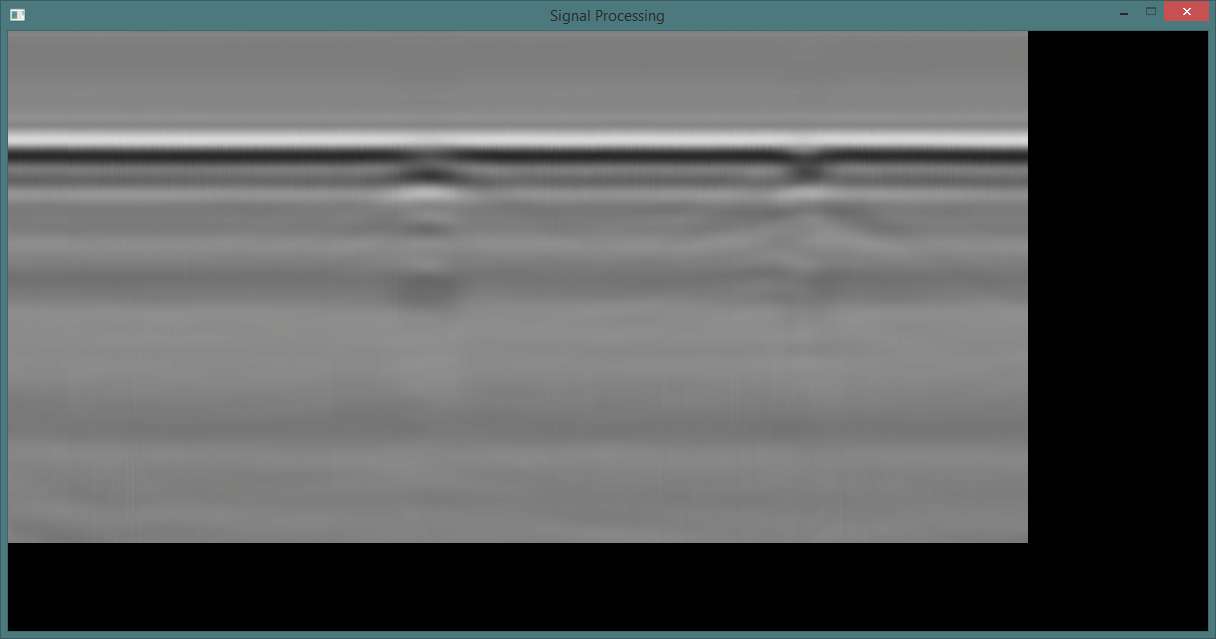
\includegraphics[width=0.8\textwidth]{7-Conclusion/raw.png}
\centering
\caption{Visualisation of raw GPR B-scan sample data}
\figlabel{raw}
\end{figure}
Preliminary progress on the detection algorithm has achieved background signal removal and primary line detection. \Figref{bgremoval} shows the background removal ability, which uses a moving average to characterise non-feature responses. Already evident from this data is the ability for the software to isolate large features and identify the approximate location of subsurface features. This is currently not sufficient progress to be able to consistently identify features or allow classification of landmines and non-landmine objects, however is sufficient to be able to clearly show visually the parabolic shapes that will be targeted and identified by the randomised Hough transfer, which are visible in \Figref{edgedetect}. Continuing work will be to progress with the detailed design path for this subsystem and implement the Hough transform to form a reduced set of metrics which will permit classification of landmines from other objects.

\begin{figure}[ht]
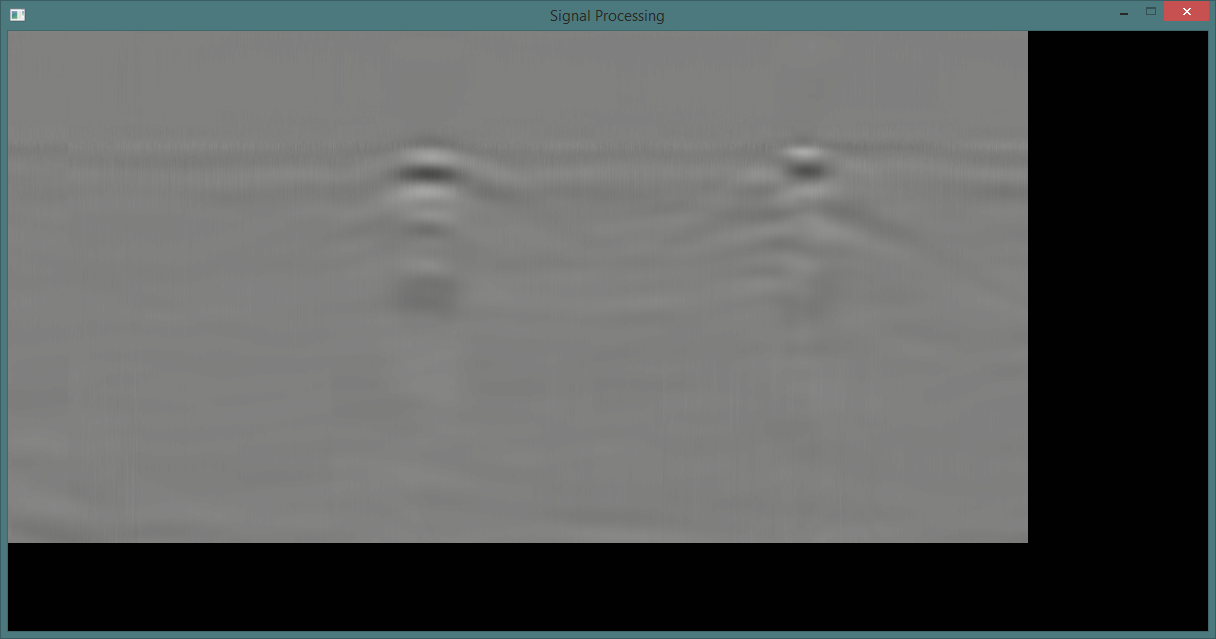
\includegraphics[width=0.8\textwidth]{7-Conclusion/bg-removed.png}
\centering
\caption{GPR B-scan data with background signal removed}
\figlabel{bgremoval}
\end{figure}

\begin{figure}[ht]
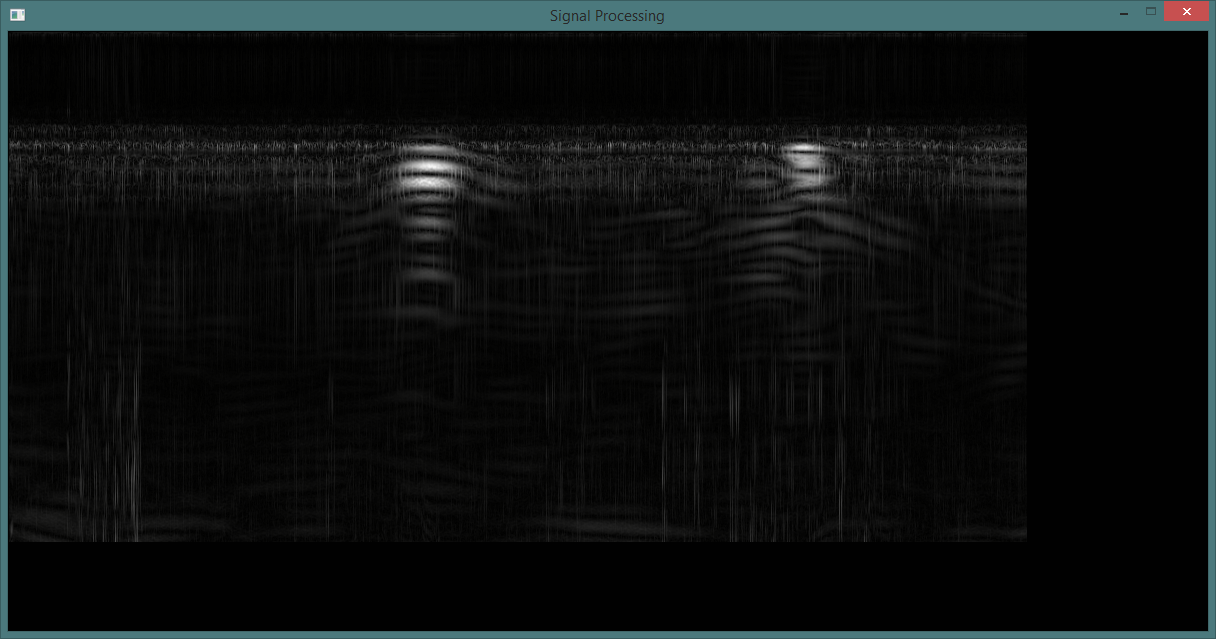
\includegraphics[width=0.8\textwidth]{7-Conclusion/edge-recognition.png}
\centering
\caption{Simple edge-detection based feature isolation}
\figlabel{edgedetect}
\end{figure}
%\subsection{Automation Systems}
Preliminary work on the autonomous path following system has commenced in desktop simulations, prior to deployment on the physical platform. This functionality is provided in the software system by the DummyHardware object, which is capable of replacing a real hardware object in the software interfaces as shown in \Figref{central}. This process will allow the development of path following routines and early detection of any bugs which may be present. Trial outputs from this system are shown in \Figref{autonomous-sim}.

\begin{figure}[ht]
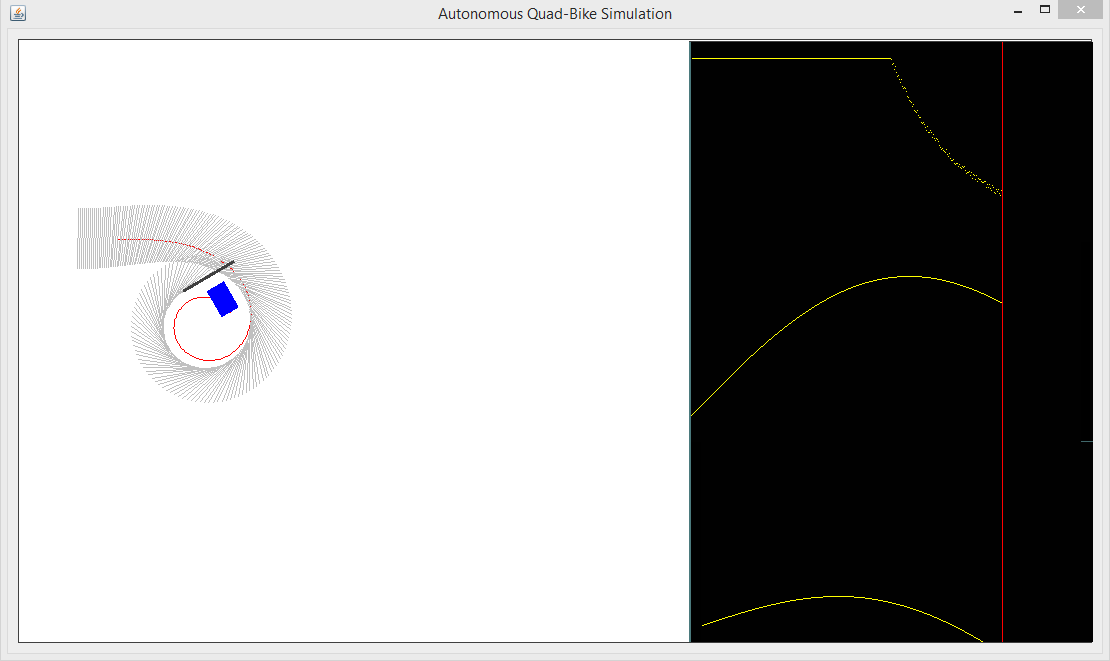
\includegraphics[width=\textwidth]{7-Conclusion/fake2.png}
\centering
\caption[Current state of the autonomous control simulation]{Current state of the autonomous control simulation, showing dummy data in logging windows alongside a plotted path.}
\figlabel{autonomous-sim}
\end{figure}
%%%%%%%%%%%%%%%%%%%%%%%%%%%%%%%%
% this sentence below is shitty. if its going to be crap then dont put it in at all.
%Future work of the project's primary objectives are discussed in the following section. 
\section{Future work}
%\textcolor{red}{Look at each objective that has not been completed yet, how will this be achieved in future (relate to the Gantt chart)}

%\textcolor{red}{What needs to be done to complete remaining objectives}

The primary region where work has been completed thus far is in the software aspects of the project, as they are capable of being developed without reliance on completion of other systems. Continuing work on the project will be to advance with current progress on the signal processing and desktop simulations of the automation and navigation controller. 
The next most-pressing objective for the signal processing and landmine detection aspects is to achieve data logging and integration of raw data collected directly from the GPR device after receiving the physical hardware from the DSTG. 
Primary connections to the project computer have been completed and the goals for the next stage are to develop an understanding of the communications protocols used by the device and link the equipment to the remainder of the project code base.
As the main control program becomes more complete, the development attention will shift towards the software for the operator control device, to ensure that all controls to the vehicle will be accessible by a remote operator, as per the project goals.

Moving into the primary work phase of the project will require a heavier emphasis on testing the quad bike platform post-evaluation, and commencing construction of the new mounts required and replacement of existing equipment which is insufficient for meeting the project goals. A significant degree of the future work program is in this platform testing, as well as operational and integration testing of the other subsystems, as shown in the project Gantt chart. 
Before testing can commence, a location to use as a testing ground needs to be organised and test programs developed, with test methodologies devised and expected outcomes noted. Securing a testing grounds is the next major challenge in the project, as this is required to allow progressing the project. 
Negotiations are currently underway for a number of potential sites to be used as a testing ground however currently nothing has been finalised.

\section{Conclusion}
Development of an autonomous platform for landmine detection and confirmation has commenced, and progress is expected to be able to return to schedule following a number of drawbacks and delays. 
Despite these factors it is anticipated that the project will be able to be completed within the allocated time frame. 
Challenges present in the project work plan that must be overcome to deliver on the project goals have been identified in the signal processing and automation subsystems, and an extensive literature review has been completed to investigate potential methods for overcoming these challenges. 
These methods were used as the driving factors for the concept design of the project. 
The proposed design for the system takes advantage of a DSTG loaned Quad bike that has pre-existing remote control functions. 
Various frame designs to mount the sensors to the platform have been considered, with emphasis placed upon the material selection and design requirements, and final designs are ready for submission to workshop staff for review.
Different electrical hardware configurations were considered for the signal processing aspects of the project.
Desktop computing hardware was determined to be the most appropriate for the central control system for the mobile platform due to the computationally intensive nature of the signal processing algorithms, and so will be used as the primary computing device on the vehicle.
Current navigation methods were investigated but focus was placed upon low speed methods that were able to accurately follow a predefined path with little deviance. 
Front steering and back steering are still aspects of navigation that require further investigation into which steering method is most applicable to this project. 



%A metal detector and a GPR will be fastened to the Quad bike through the use of PVC and fibreglass constructed frame to minmise 


%% OI PETER
% my summary of the lit review - summarises what happened in OUR lit review. doesnt go into specifics about decisions because we've already got that. this is a big report so we need to keep a broader scope here


%The DSTG expressed interest in the risk reduction and accuracy improvements over current detection methods through the use of multi-sensor equipment mounted on an autonomous platform. 
%Literature reviews allowed for current state-of-the-art landmine detection methods to be reviewed as well as automation and navigation methods for unmanned platforms. 
%The challenges and shortcomings for each system were used as the driving factors for the concept designs. 
%The most favourable aspects of each proposed design was selected resulting in a full system preliminary design. This design was further developed to produce the detailed design. 

Future work for the coming term involves: taking delivery of the platform, construction of the sensor mount, procurement of the metal detector, sensor testing, and whole system testing. 
Testing locations are required and negotiations are currently underway to finalise access arrangements to these facilities. 





\end{document}